\documentclass[12pt, a4paper]{article}

\usepackage{array}
\usepackage[portuguese]{babel}
\usepackage{float}
\usepackage[a4paper, margin=2cm]{geometry}
\usepackage{graphicx}
\usepackage{hyperref}
\usepackage{pdfpages}
\usepackage{setspace}

\title{\textbf{Interface Pessoa-Máquina \\ \large Trabalho Prático -- Fase II}}
\date{4 de maio de 2025}
\author{Grupo 12 \\
    \url{https://github.com/UMinho-ENGINF-IPM/trabalho-pr-tico-gp25_12}}

\begin{document}

\begin{center}
    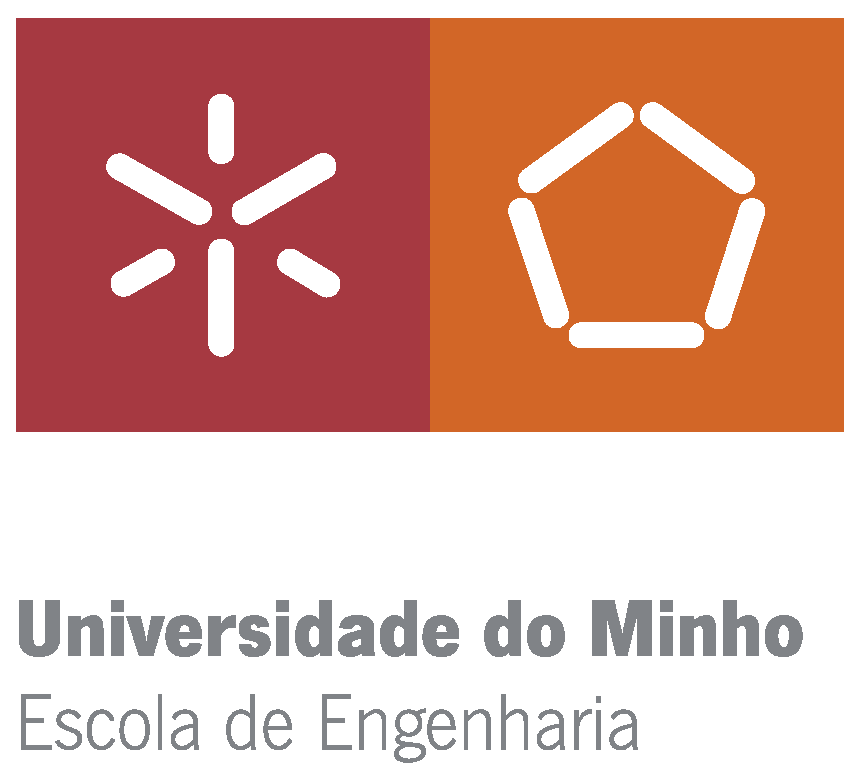
\includegraphics[width=0.25\textwidth]{res/cover/school-of-engineering.eps}
\end{center}

{\let\newpage\relax\maketitle}
\maketitle
\thispagestyle{empty}

\chardef\_=`_
\onehalfspacing
\setlength{\parskip}{\baselineskip}
\setlength{\intextsep}{2\baselineskip}
\setlength\belowcaptionskip{-\baselineskip}
\setlength{\parindent}{0pt}
\def\arraystretch{1.5}

\vspace{2cm}
\begin{center}
    \begin{tabular}{>{\centering}p{0.25\textwidth}
                    >{\centering}p{0.25\textwidth}
                    >{\centering\arraybackslash}p{0.25\textwidth}}
        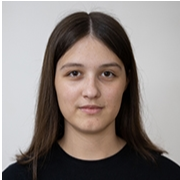
\includegraphics[width=3.5cm]{res/cover/A104437.png} &
        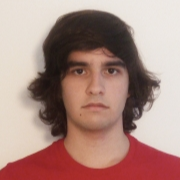
\includegraphics[width=3.5cm]{res/cover/A104348.png} &
        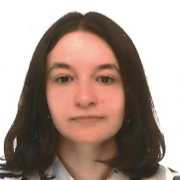
\includegraphics[width=3.5cm]{res/cover/A104263.png}  \\

        Ana Oliveira & Humberto Gomes & Inês Marques \\
        A104437      & A104348        & A104263
    \end{tabular}

    \begin{tabular}{>{\centering}p{0.25\textwidth}
                    >{\centering\arraybackslash}p{0.25\textwidth}}
        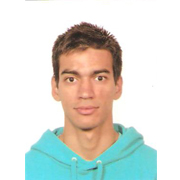
\includegraphics[width=3.5cm]{res/cover/A76350.jpg} &
        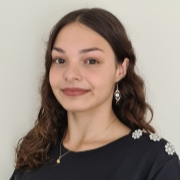
\includegraphics[width=3.5cm]{res/cover/A104179.png} \\

        Rafael Vilas Boas & Sara Lopes \\
        A76350            & A104179
    \end{tabular}
\end{center}

\begin{abstract}
    \noindent
\end{abstract}

\section{Alterações ao Modelo da Interface}

Na fase anterior deste trabalho prático, construiu-se, em Figma \cite{figma}, um modelo da interface
a implementar. Apesar de uma boa avaliação nesta fase, a docência da UC de Interface Pessoa-Máquina
reparou em alguns aspetos que podiam ser melhorados. Nesta secção, apresentam-se as mudanças que
foram feitas ao modelo da interface devido tanto aos comentários dos docentes como a outros aspetos
que o grupo de trabalho se apercebeu que podiam ser melhorados.

Em primeiro lugar, a página ``Iniciar Sessão'' não é ideal para a prevenção de erros: é possível que
o utilizador submeta parcialmente as suas credenciais (apenas o seu endereço eletrónico ou apenas a
sua palavra-passe), e o sistema reagirá com um erro. Para prevenir este erro, deve ser impossível
que um utilizador submeta as suas credenciais até as escrever todas. Logo, na nova versão do modelo
da interface, o botão de submissão de credenciais encontra-se desativado até o utilizador escrever
tanto o seu endereço eletrónico como a sua palavra-passe, como mostra a figura abaixo:

{\color{red} TODO - figura}

É importante que o utilizador saiba por que este botão se encontra desativado, pelo que, tal como
foi feito em outros botões na interface, uma \emph{tooltip} foi utilizada para justificar por que
não é possível interagir com o botão:

{\color{red} TODO - figura}

Ademais, na página ``Resolver Problemas'', o título da página foi removido, e substituído por uma
barra de pesquisa. Em primeiro lugar, o título da página não era necessário, visto que o utilizador
já sabe em que página se encontra olhando para a hiperligação realçada na barra de navegação.
Depois, o espaço que se ganha na barra lateral com a remoção deste título pode ser usado uma barra
de pesquisa, um elemento muito útil para procurar alunos em grandes listas de problemas (o cenário 1
aponta para 45 alunos sem turnos atribuídos).

{\color{red} TODO - figura}

Por último, uma sugestão da docência de Interface Pessoa-Máquina foi a eliminação da página
``Publicar Horários'', sendo estes atualizados sempre que o diretor de curso faz uma alteração. No
entanto, não consideramos esta solução viável, visto que o diretor de curso pode desejar colocar os
horários dos alunos em estados intermédios sem que estes os vejam. Por exemplo, pode desejar remover
vários alunos dos seus turnos, para os adicionar a outros turnos da mesma UC, assim, por exemplo,
abrindo vagas em turnos mais procurados. No entanto, reparou-se que é importante realçar quando as
mudanças feitas pelo diretor de curso ainda não são públicas. Por esse motivo, tal como foi feito
para o ícone de notificações, quando há alterações por publicar, um pequeno círculo é adicionado ao
canto superior direito da hiperligação para a página "Publicar Horários", como mostra a figura
abaixo:

{\color{red} TODO - figura}

\section{Componentes Implementados}

\section{Páginas Implementadas}

\section{Tecnologias Utilizadas}

\section{Conclusão e Trabalho Futuro}

\begingroup
\section{Bibliografia}
\renewcommand{\section}[2]{}

\begin{thebibliography}{9}
    \bibitem{figma}
        ``Figma: Collaborative Interface Design Tool.''. Figma. Accessed: Mar. 13, 2025. [Online.]
        Available: \url{https://www.figma.com/}
\end{thebibliography}
\endgroup

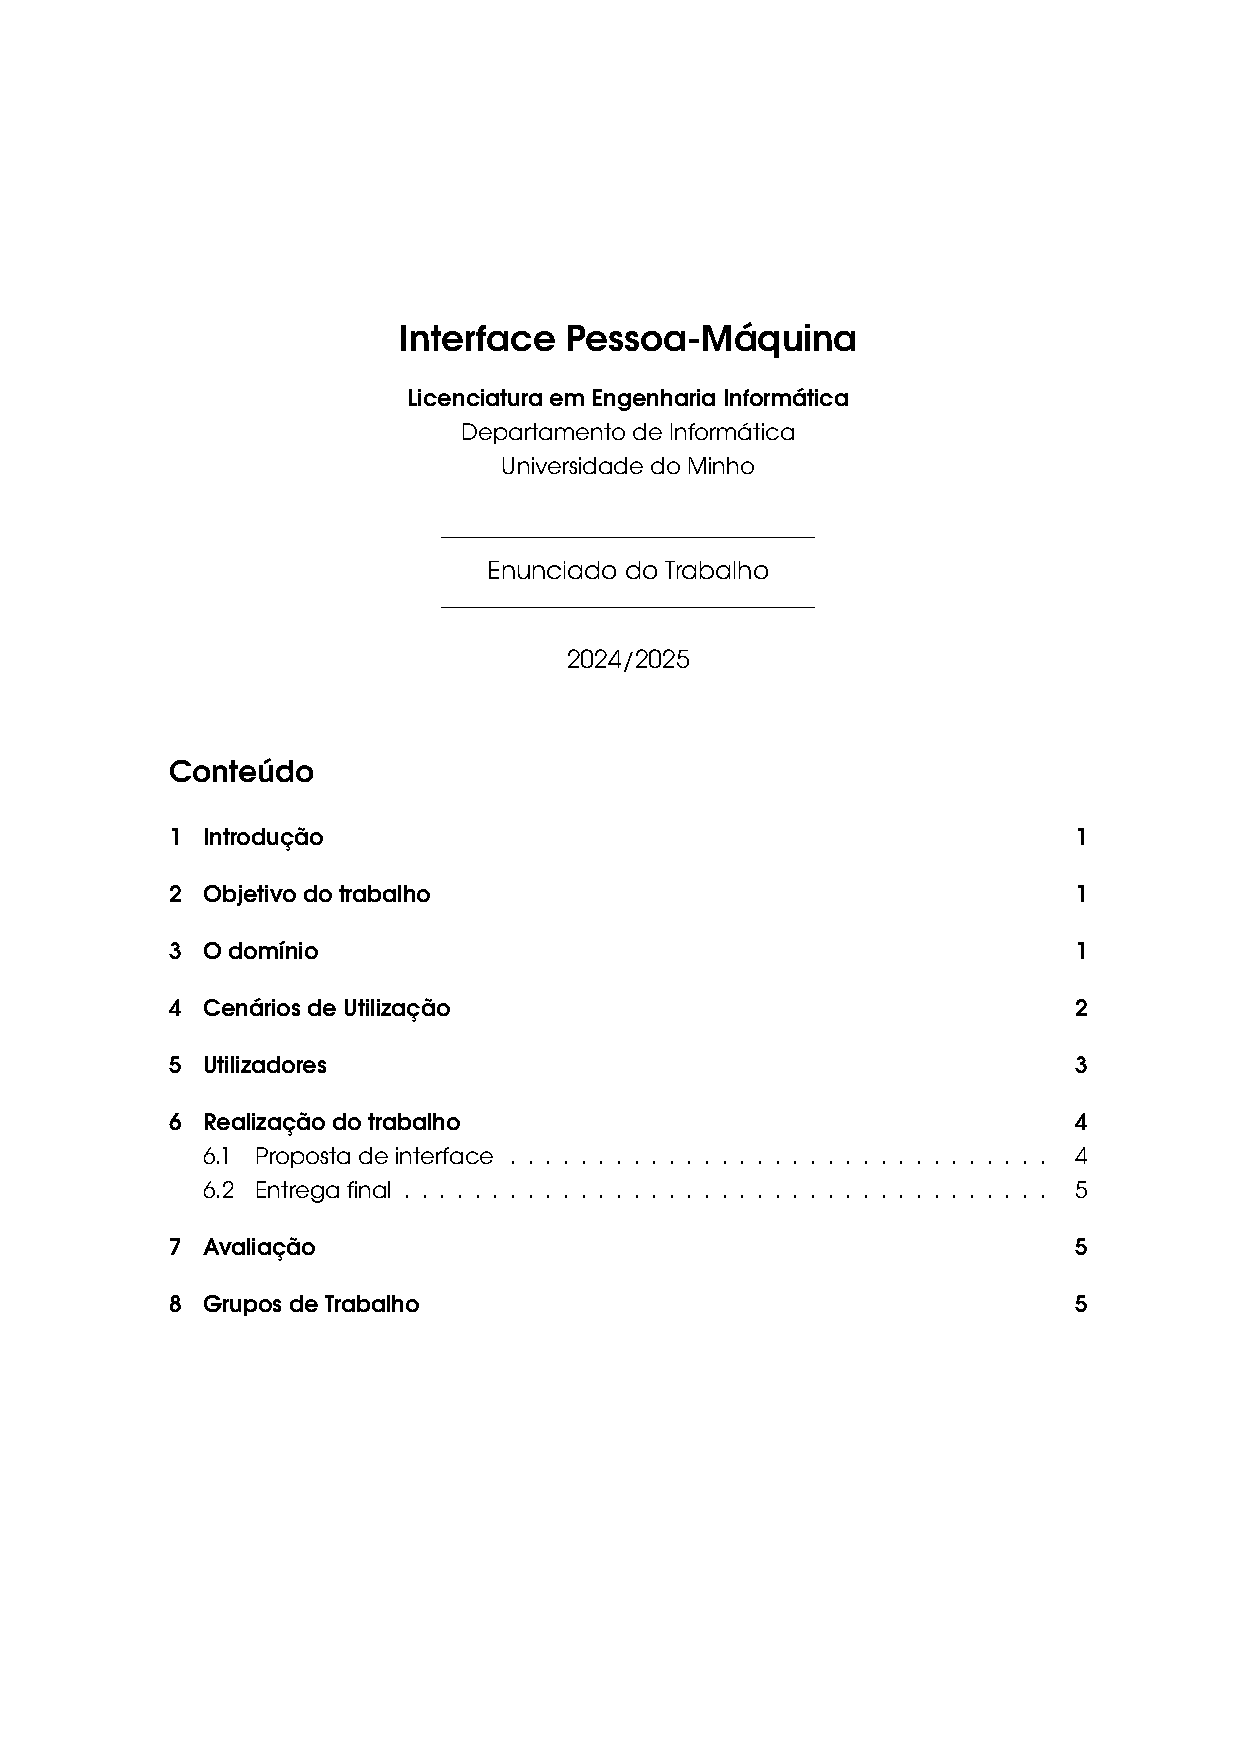
\includepdf[pages=1,pagecommand=\section{Anexo -- Enunciado do Trabalho}\thispagestyle{empty}]
    {../Assignment.pdf}
\includepdf[pages=2-]{../Assignment.pdf}

\end{document}
